\section{Experiments}

\subsection{Multi-task learning}

\subsubsection{CLEVR tasks}
\vm{Will have to rephrase this in accordance with Jayram's definition.}

We have trained SAMNet using MI-Prometheus~\cite{kornuta2018accelerating}, a framework based on PyTorch~\cite{paszke2017automatic}, using the training set of the condition A of the CLEVR dataset (CLEVR-CoGenT)~\cite{johnson2017clevr}.
For all experiments, the training procedure is as follows: we train the model for 20 epochs on 90\% of the training set of CoGenT. We keep the remaining 10\% for validating the model at every epoch, and use the original validation sets (CoGenT-A  \& -B) as test sets. We used NVIDIA's GeForce GTX TITAN X GPUs.

We consider as task groups the question categories defined by the authors: \textit{Exist}, \textit{Count}, \textit{CompareInteger}, \textit{CompareAttribute}, \textit{QueryAttribute}. In order to investigate the potential benefits of multi-task learning, we conducted the following experiments:

\begin{itemize}
	\item We first trained SAMNet on a single task group $t$, and tested on this same task group. These 5 experiments (one per task group) fit into the traditional Deep Learning procedure of training and testing on the same task, or on samples drawn from the same distribution over a common input domain (single-task learning).
	\item Following, we trained SAMNet on all task groups jointly, and evaluated its performance on each group $t$ separately. The underlying hypothesis for this experiment is that learning jointly on all task groups would improve the performance on each task group.
	\item Finally, for each task group $t$, we trained SAMNet on all tasks but $t$, and tested its performance on $t$. These experiments steer away from single / multi-task training and rather fall under the Domain Adaptation setting, categorized as \emph{transductive} transfer learning in \cite{pan2009survey}.
\end{itemize}

\begin{figure}[!t]
	\centering
	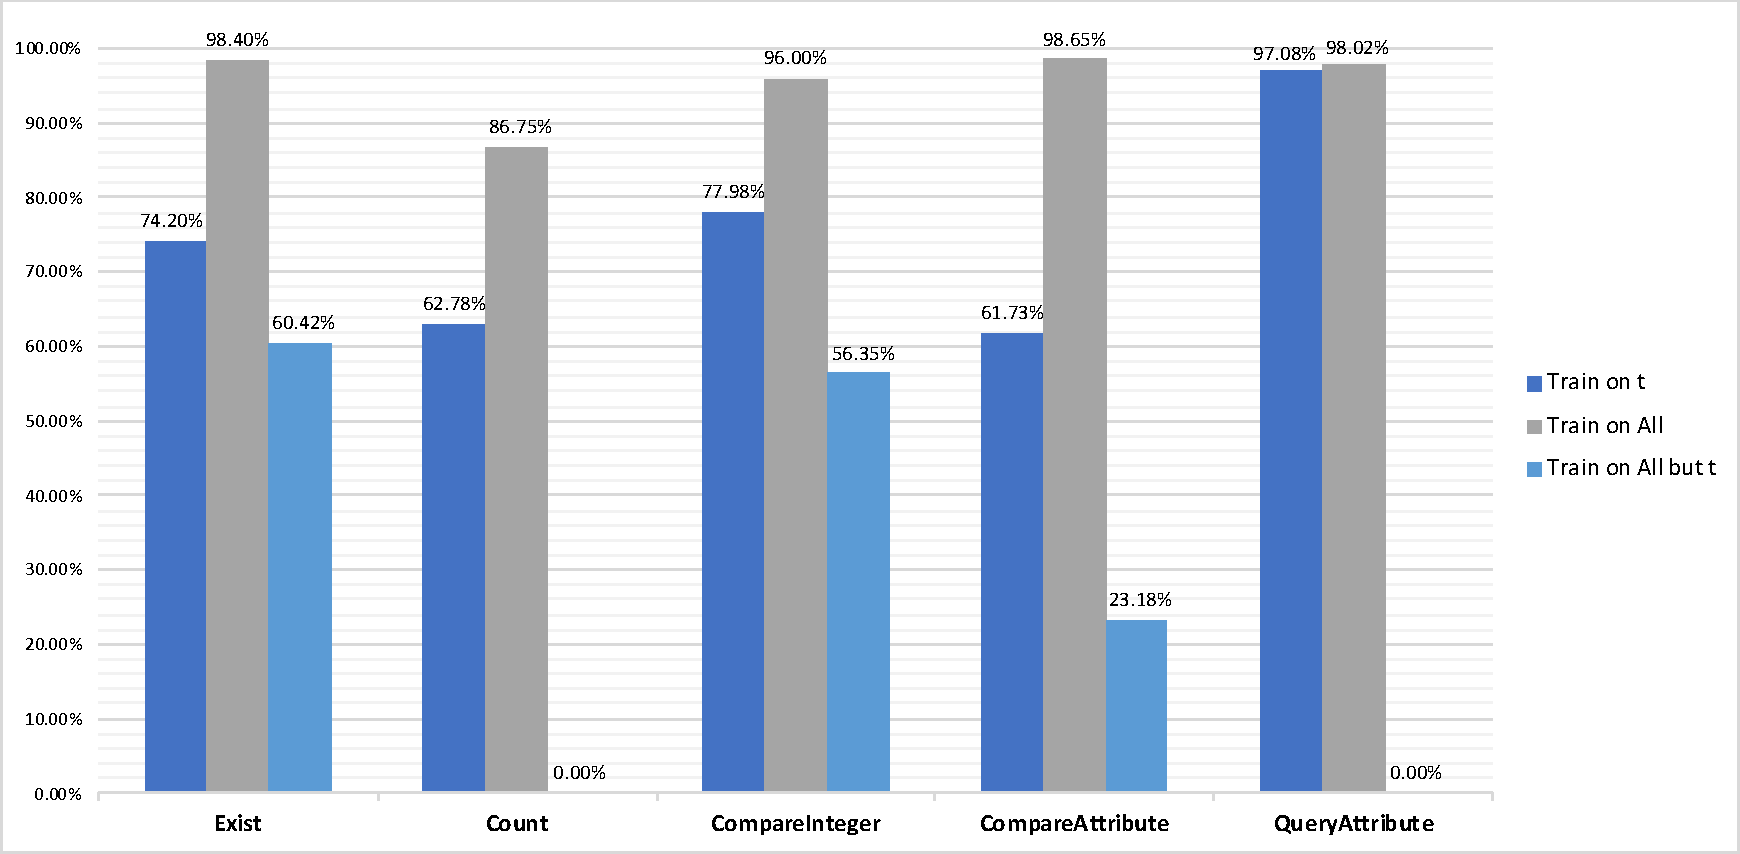
\includegraphics[width=0.5\textwidth]{img/charts/CoGenT_results.pdf}
	\caption{CLEVR-CoGenT accuracies for all 5 tasks $t$ when training on $t$ only, training on all tasks jointly and training on all tasks but $t$. For all experiments, the validation and test sets are identical.}
	\label{fig:CoGenT-results}
\end{figure}

The results of these experiments are available in \Fig{fig:CoGenT-results}. The complete set of results is available in Appendix \ref{sec:full-cogent-results}.


Looking at \Fig{fig:CoGenT-results}, we observe that single-task learning results in better-than-average performance on the same task. \textit{Exist}, \textit{CompareInteger} and \textit{CompareInteger} are binary tasks (\textit{yes} or \textit{no}); \textit{Count} has for corresponding labels the digits 0 through 10 (11 labels in total, hence a random agent would obtain ~9.1\% accuracy) and \textit{QueryAttribute} has for labels the set of object attributes values (15 labels, hence an an accuracy of 6.7\% would be associated with chance). In that perspective, SAMNet does well on \textit{Count} and \textit{QueryAttribute}, but poorer on the 3 other tasks.

Nonetheless, significant accuracy gains are observed when training jointly on all 5 tasks. We indeed observe improvements ranging from 18 points to 37 points on 4 out of 5 tasks. \textit{QueryAttribute} does not benefit from such an improvement, only seeing an increase of one point in terms of test accuracy. One could qualify this task as \textit{self-sufficient}, as single- and multi-task learning performance are close.
These accuracy improvements thus suggest that related tasks benefit from joint training, i.e. \emph{the whole is greater than the sum of the parts}. One further set of experiments here could favor the granularity of the observed improvements, by jointly training on $t$ and all possible subsets of the remaining 4 tasks. We hypothesize that the improvements on e.g. \textit{Exist} would mostly originate from training jointly on \textit{CompareAttribute} and \textit{CompareInteger} since all 3 tasks share the same output space (i.e. labels domain).
% 5 x 2^4 = 80 experiments to get that granularity.

Finally, the "all-tasks-but-$t$" experiments demonstrate that while task groups are related, one does not subsume another in terms of learning. Indeed, we can observe that for \textit{CompareAttribute}, while \textit{Exist} and \textit{CompareInteger} share the same output space, including them and holding out \textit{CompareAttribute} from the training set results in poor accuracy. We also observe accuracy of zero for \textit{Count} and \textit{QueryAttribute}. This is due to these tasks having distinct labels domains, which do not overlap with the other tasks labels domain. Thus, if holding out samples from \textit{Count} during training, a model will not be able to learn to predict the corresponding labels ('0' through '10').

 
A final set of experiment, for which the results are available in Appendix \ref{sec:full-cogent-results}, finetuned the model trained on all tasks on each task $t$ respectively. Given that the initial pretraining on all tasks, we were interested in the tradeoff between the significance of the performance gain, if any, on the finetuned task and the performance drop, if any, on the other tasks. Finetuning did not demonstrate a statistically meaningful benefit (except for \textit{Count}, where the accuracy increased by 1.5 pt) without hurting performance on the other tasks. Nevertheless, these experiments leave open the possibility that the training method for multi-task training could potentially benefit from using weighted sampling towards the tail end with more emphasis on samples from less performing task groups. Recent work~\cite{guo2018dynamic, kendall2018multi} in this direction has been done, although seems to weigh the tasks rather than the samples.